
\chapter{Basic Principles}
\label{chapter:basics}

This chapter contains a short introduction to the basic principles of digital
circuit synthesis.

\section{Levels of Abstraction}

Digital circuits can be represented at different levels of abstraction.
During the design process a circuit is usually first specified using a higher
level abstraction. Implementation can then be understood as finding a
functionally equivalent representation at a lower abstraction level.  When
this is done automatically using software, the term {\it synthesis} is used.

So synthesis is the automatic conversion of a high-level representation of a
circuit to a functionally equivalent low-level representation of a circuit.
Figure~\ref{fig:Basics_abstractions} lists the different levels of abstraction
and how they relate to different kinds of synthesis.

\begin{figure}[b!]
	\hfil
	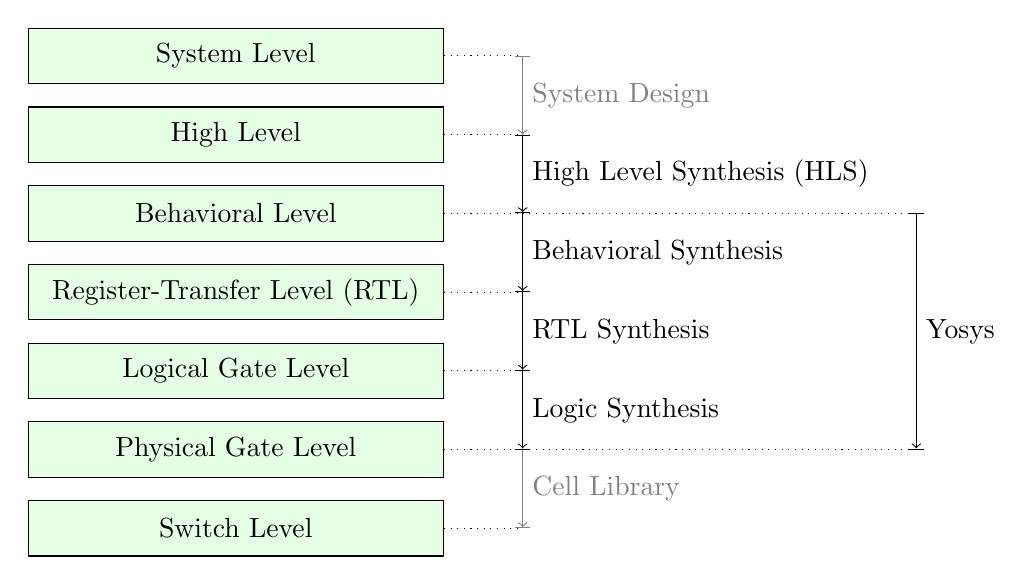
\begin{tikzpicture}
			\tikzstyle{lvl} = [draw, fill=green!10, rectangle, minimum height=2em, minimum width=15em]
			\node[lvl] (sys) {System Level};
			\node[lvl] (hl) [below of=sys] {High Level};
			\node[lvl] (beh) [below of=hl] {Behavioral Level};
			\node[lvl] (rtl) [below of=beh] {Register-Transfer Level (RTL)};
			\node[lvl] (lg) [below of=rtl] {Logical Gate Level};
			\node[lvl] (pg) [below of=lg] {Physical Gate Level};
			\node[lvl] (sw) [below of=pg] {Switch Level};

			\draw[dotted] (sys.east)  -- ++(1,0) coordinate (sysx);
			\draw[dotted] (hl.east)  -- ++(1,0) coordinate (hlx);
			\draw[dotted] (beh.east) -- ++(1,0) coordinate (behx);
			\draw[dotted] (rtl.east) -- ++(1,0) coordinate (rtlx);
			\draw[dotted] (lg.east)  -- ++(1,0) coordinate (lgx);
			\draw[dotted] (pg.east)  -- ++(1,0) coordinate (pgx);
			\draw[dotted] (sw.east)  -- ++(1,0) coordinate (swx);

			\draw[gray,|->] (sysx) -- node[right] {System Design} (hlx);
			\draw[|->|] (hlx) -- node[right] {High Level Synthesis (HLS)} (behx);
			\draw[->|] (behx) -- node[right] {Behavioral Synthesis} (rtlx);
			\draw[->|] (rtlx) -- node[right] {RTL Synthesis} (lgx);
			\draw[->|] (lgx) -- node[right] {Logic Synthesis} (pgx);
			\draw[gray,->|] (pgx) -- node[right] {Cell Library} (swx);

			\draw[dotted] (behx) -- ++(5,0) coordinate (a);
			\draw[dotted] (pgx) -- ++(5,0) coordinate (b);
			\draw[|->|] (a) -- node[right] {Yosys} (b);
	\end{tikzpicture}
	\caption{Different levels of abstraction and synthesis.}
	\label{fig:Basics_abstractions}
\end{figure}

Regardless of the way a lower level representation of a circuit is
obtained (synthesis or manual design), the lower level representation is usually
verified by comparing simulation results of the lower level and the higher level
representation \footnote{In recent years formal equivalence 
checking also became an important verification method for validating RTL and 
lower abstraction representation of the design.}.
Therefore even if no synthesis is used, there must still be a simulatable
representation of the circuit in all levels to allow for verification of the
design.

Note: The exact meaning of terminology such as ``High-Level'' is of course not
fixed over time. For example the HDL ``ABEL'' was first introduced in 1985 as ``A High-Level
Design Language for Programmable Logic Devices'' \cite{ABEL}, but would not
be considered a ``High-Level Language'' today.

\subsection{System Level}

The System Level abstraction of a system only looks at its biggest building
blocks like CPUs and computing cores. At this level the circuit is usually described
using traditional programming languages like C/C++ or Matlab. Sometimes special
software libraries are used that are aimed at simulation circuits on the system
level, such as SystemC.

Usually no synthesis tools are used to automatically transform a system level
representation of a circuit to a lower-level representation. But system level
design tools exist that can be used to connect system level building blocks.

The IEEE 1685-2009 standard defines the IP-XACT file format that can be used to
represent designs on the system level and building blocks that can be used in
such system level designs. \cite{IP-XACT}

\subsection{High Level}

The high-level abstraction of a system (sometimes referred to as {\it
algorithmic} level) is also often represented using traditional programming
languages, but with a reduced feature set. For example when representing a
design at the high level abstraction in C, pointers can only be used to mimic
concepts that can be found in hardware, such as memory interfaces. Full
featured dynamic memory management is not allowed as it has no corresponding
concept in digital circuits.

Tools exist to synthesize high level code (usually in the form of C/C++/SystemC
code with additional metadata) to behavioural HDL code (usually in the form of
Verilog or VHDL code). Aside from the many commercial tools for high level synthesis
there are also a number of FOSS tools for high level synthesis
\citeweblink{C_to_Verilog} \citeweblink{LegUp}.

\subsection{Behavioural Level}

At the behavioural abstraction level a language aimed at hardware description such
as Verilog or VHDL is used to describe the circuit, but so-called {\it behavioural
modelling} is used in at least part of the circuit description. In behavioural
modelling there must be a language feature that allows for imperative programming to be used to
describe data paths and registers. This is the {\tt always}-block in Verilog and
the {\tt process}-block in VHDL.

In behavioural modelling, code fragments are provided together with a {\it
sensitivity list}; a list of signals and conditions. In simulation, the code
fragment is executed whenever a signal in the sensitivity list changes its
value or a condition in the sensitivity list is triggered. A synthesis tool
must be able to transfer this representation into an appropriate datapath followed
by the appropriate types of register.

For example consider the following verilog code fragment:

\begin{lstlisting}[numbers=left,frame=single,language=Verilog]
always @(posedge clk)
	y <= a + b;
\end{lstlisting}

In simulation the statement \lstinline[language=Verilog]{y <= a + b} is executed whenever
a positive edge on the signal \lstinline[language=Verilog]{clk} is detected. The synthesis
result however will contain an adder that calculates the sum \lstinline[language=Verilog]{a + b}
all the time, followed by a d-type flip-flop with the adder output on its D-input and the
signal \lstinline[language=Verilog]{y} on its Q-output.

Usually the imperative code fragments used in behavioural modelling can contain
statements for conditional execution (\lstinline[language=Verilog]{if}- and
\lstinline[language=Verilog]{case}-statements in Verilog) as well as loops,
as long as those loops can be completely unrolled.

Interestingly there seems to be no other FOSS Tool that is capable of
performing Verilog or VHDL behavioural syntheses besides Yosys (see
App.~\ref{chapter:sota}).

\subsection{Register-Transfer Level (RTL)}

On the Register-Transfer Level the design is represented by combinatorial data
paths and registers (usually d-type flip flops). The following verilog code fragment
is equivalent to the previous verilog example, but is in RTL representation:

\begin{lstlisting}[numbers=left,frame=single,language=Verilog]
assign tmp = a + b;       // combinatorial data path

always @(posedge clk)     // register
	y <= tmp;
\end{lstlisting}

A design in RTL representation is usually stored using HDLs like Verilog and VHDL. But only
a very limited subset of features is used, namely minimalistic {\tt always}-blocks (Verilog)
or {\tt process}-blocks (VHDL) that model the register type used and unconditional assignments
for the datapath logic. The use of HDLs on this level simplifies simulation as no additional
tools are required to simulate a design in RTL representation.

Many optimizations and analyses can be performed best at the RTL level. Examples include FSM
detection and optimization, identification of memories or other larger building blocks
and identification of shareable resources.

Note that RTL is the first abstraction level in which the circuit is represented as a
graph of circuit elements (registers and combinatorical cells) and signals. Such a graph,
when encoded as list of cells and connections, is called a netlist.

RTL synthesis is easy as each circuit node element in the netlist can simply be replaced
with an equivalent gate-level circuit. However, usually the term {\it RTL synthesis} does
not only refer to synthesizing an RTL netlist to a gate level netlist but also to performing
a number of highly sophisticated optimizations within the RTL representation, such as
the examples listed above.

A number of FOSS tools exist that can perform isolated tasks within the domain of RTL
synthesis steps. But there seems to be no FOSS tool that covers a wide range of RTL
synthesis operations.

\subsection{Logical Gate Level}

At the logical gate level the design is represented by a netlist that uses only
cells from a small number of single-bit cells, such as basic logic gates (AND,
OR, NOT, XOR, etc.) and registers (usually D-Type Flip-flops).

A number of netlist formats exists that can be used on this level, e.g.~the Electronic Design
Interchange Format (EDIF), but for ease of simulation often a HDL netlist is used. The latter
is a HDL file (Verilog or VHDL) that only uses the most basic language constructs for instantiation
and connecting of cells.

There are two challenges in logic synthesis: First finding opportunities for optimizations
within the gate level netlist and second the optimal (or at least good) mapping of the logic
gate netlist to an equivalent netlist of physically available gate types.

The simplest approach to logic synthesis is {\it two-level logic synthesis}, where a logic function
is converted into a sum-of-products representation, e.g.~using a Karnaugh map.
This is a simple approach, but has exponential worst-case effort and cannot make efficient use of
physical gates other than AND/NAND-, OR/NOR- and NOT-Gates.

Therefore modern logic synthesis tools utilize much more complicated {\it multi-level logic
synthesis} algorithms \cite{MultiLevelLogicSynth}. Most of these algorithms convert the
logic function to a Binary-Decision-Diagram (BDD) or And-Inverter-Graph (AIG) and work from that
representation. The former has the advantage that it has a unique normalized form. The latter has
much better worst case performance and is therefore better suited for the synthesis of large
logic functions.

Good FOSS tools exists for multi-level logic synthesis \citeweblink{ABC}
\citeweblink{AIGER} \citeweblink{MVSIS}.

Yosys contains basic logic synthesis functionality but can also use ABC
\citeweblink{ABC} for the logic synthesis step. Using ABC is recommended.

\subsection{Physical Gate Level}

On the physical gate level only gates are used that are physically available on
the target architecture. In some cases this may only be NAND, NOR and NOT gates as well as
D-Type registers. In other cases this might include cells that are more complex than the cells
used at the logical gate level (e.g.~complete half-adders). In the case of an FPGA-based
design the physical gate level representation is a netlist of LUTs with optional output
registers, as these are the basic building blocks of FPGA logic cells.

For the synthesis tool chain this abstraction is usually the lowest level. In
case of an ASIC-based design the cell library might contain further information on
how the physical cells map to individual switches (transistors).

\subsection{Switch Level}

A switch level representation of a circuit is a netlist utilizing single transistors as cells.
Switch level modelling is possible in Verilog and VHDL, but is seldom used in modern designs,
as in modern digital ASIC or FPGA flows the physical gates are considered the atomic build blocks
of the logic circuit.

\subsection{Yosys}

Yosys is a Verilog HDL synthesis tool. This means that it takes a behavioural
design description as input and generates an RTL, logical gate or physical gate
level description of the design as output.  Yosys' main strengths are behavioural
and RTL synthesis. A wide range of commands (synthesis passes) exist
within Yosys that can be used to perform a wide range of synthesis tasks within
the domain of behavioural, rtl and logic synthesis. Yosys is designed to be
extensible and therefore is a good basis for implementing custom synthesis
tools for specialised tasks.

\section{Features of Synthesizable Verilog}

The subset of Verilog \cite{Verilog2005} that is synthesizable is specified in
a separate IEEE standards document, the IEEE standard 1364.1-2002 \cite{VerilogSynth}.
This standard also describes how certain language constructs are to be interpreted in
the scope of synthesis.

This section provides a quick overview of the most important features of
synthesizable Verilog, structured in order of increasing complexity.

\subsection{Structural Verilog}

{\it Structural Verilog} (also known as {\it Verilog Netlists}) is a Netlist in
Verilog syntax. Only the following language constructs are used in this case:

\begin{itemize}
\item Constant values
\item Wire and port declarations
\item Static assignments of signals to other signals
\item Cell instantiations
\end{itemize}

Many tools (especially at the back end of the synthesis chain) only support
structural verilog as input. ABC is an example of such a tool. Unfortunately
there is no standard specifying what {\it Structural Verilog} actually is,
leading to some confusion about what syntax constructs are supported in
structural verilog when it comes to features such as attributes or multi-bit
signals.

\subsection{Expressions in Verilog}

In all situations where Verilog accepts a constant value or signal name, 
expressions using arithmetic operations such as
\lstinline[language=Verilog]{+}, \lstinline[language=Verilog]{-} and \lstinline[language=Verilog]{*},
boolean operations such as
\lstinline[language=Verilog]{&} (AND), \lstinline[language=Verilog]{|} (OR) and \lstinline[language=Verilog]{^} (XOR)
and many others (comparison operations, unary operator, etc.) can also be used.

During synthesis these operators are replaced by cells that implement the respective function.

Many FOSS tools that claim to be able to process Verilog in fact only support
basic structural verilog and simple expressions. Yosys can be used to convert
full featured synthesizable verilog to this simpler subset, thus enabling such
applications to be used with a richer set of Verilog features.

\subsection{Behavioural Modelling}

Code that utilizes the Verilog {\tt always} statement is using {\it Behavioural
Modelling}. In behavioural modelling, a circuit is described by means of imperative
program code that is executed on certain events, namely any change, a rising
edge, or a falling edge of a signal. This is a very flexible construct during
simulation but is only synthesizable when one of the following is modelled:

\begin{itemize}
\item {\bf Asynchronous or latched logic} \\
In this case the sensitivity list must contain all expressions that are used within
the {\tt always} block. The syntax \lstinline[language=Verilog]{@*} can be used
for these cases. Examples of this kind include:

\begin{lstlisting}[numbers=left,frame=single,language=Verilog]
// asynchronous
always @* begin
	if (add_mode)
		y <= a + b;
	else
		y <= a - b;
end

// latched
always @* begin
	if (!hold)
		y <= a + b;
end
\end{lstlisting}

Note that latched logic is often considered bad style and in many cases just
the result of sloppy HDL design. Therefore many synthesis tools generate warnings
whenever latched logic is generated.

\item {\bf Synchronous logic (with optional synchronous reset)} \\
This is logic with d-type flip-flops on the output. In this case the sensitivity
list must only contain the respective clock edge. Example:
\begin{lstlisting}[numbers=left,frame=single,language=Verilog]
// counter with synchronous reset
always @(posedge clk) begin
	if (reset)
		y <= 0;
	else
		y <= y + 1;
end
\end{lstlisting}

\item {\bf Synchronous logic with asynchronous reset} \\
This is logic with d-type flip-flops with asynchronous resets on the output. In
this case the sensitivity list must only contain the respective clock and reset edges.
The values assigned in the reset branch must be constant. Example:
\begin{lstlisting}[numbers=left,frame=single,language=Verilog]
// counter with asynchronous reset
always @(posedge clk, posedge reset) begin
	if (reset)
		y <= 0;
	else
		y <= y + 1;
end
\end{lstlisting}
\end{itemize}

Many synthesis tools support a wider subset of flip-flops that can be modelled
using {\tt always}-statements (including Yosys). But only the ones listed above
are covered by the Verilog synthesis standard and when writing new designs one
should limit herself or himself to these cases.

In behavioural modelling, blocking assignments (=) and non-blocking assignments
(<=) can be used. The concept of blocking vs.~non-blocking assignment is one
of the most misunderstood constructs in Verilog \cite{Cummings00}.

The blocking assignment behaves exactly like an assignment in any imperative
programming language, while with the non-blocking assignment the right hand side
of the assignment is evaluated immediately but the actual update of the left
hand side register is delayed until the end of the time-step. For example the Verilog
code \lstinline[language=Verilog]{a <= b; b <= a;} exchanges the values of
the two registers. See Sec.~\ref{sec:blocking_nonblocking} for a more
detailed description of this behaviour.

\subsection{Functions and Tasks}

Verilog supports {\it Functions} and {\it Tasks} to bundle statements that are
used in multiple places (similar to {\it Procedures} in imperative programming).
Both constructs can be implemented easily by substituting the function/task-call
with the body of the function or task.

\subsection{Conditionals, Loops and Generate-Statements}

Verilog supports \lstinline[language=Verilog]{if-else}-statements and
\lstinline[language=Verilog]{for}-loops inside \lstinline[language=Verilog]{always}-statements.

It also supports both features in \lstinline[language=Verilog]{generate}-statements
on the module level. This can be used to selectively enable or disable parts of the
module based on the module parameters (\lstinline[language=Verilog]{if-else})
or to generate a set of similar subcircuits (\lstinline[language=Verilog]{for}).

While the \lstinline[language=Verilog]{if-else}-statement
inside an always-block is part of behavioural modelling, the three other cases
are (at least for a synthesis tool) part of a built-in macro processor. Therefore it must
be possible for the synthesis tool to completely unroll all loops and evaluate the
condition in all \lstinline[language=Verilog]{if-else}-statement in
\lstinline[language=Verilog]{generate}-statements using const-folding.

Examples for this can be found in Fig.~\ref{fig:StateOfTheArt_for} and
Fig.~\ref{fig:StateOfTheArt_gen} in App.~\ref{chapter:sota}.

\subsection{Arrays and Memories}

Verilog supports arrays. This is in general a synthesizable language feature.
In most cases arrays can be synthesized by generating addressable memories.
However, when complex or asynchronous access patterns are used, it is not
possible to model an array as memory. In these cases the array must
be modelled using individual signals for each word and all accesses to the array
must be implemented using large multiplexers.

In some cases it would be possible to model an array using memories, but it
is not desired. Consider the following delay circuit:
\begin{lstlisting}[numbers=left,frame=single,language=Verilog]
module (clk, in_data, out_data);

parameter BITS = 8;
parameter STAGES = 4;

input clk;
input [BITS-1:0] in_data;
output [BITS-1:0] out_data;
reg [BITS-1:0] ffs [STAGES-1:0];

integer i;
always @(posedge clk) begin
	ffs[0] <= in_data;
	for (i = 1; i < STAGES; i = i+1)
		ffs[i] <= ffs[i-1];
end

assign out_data = ffs[STAGES-1];

endmodule
\end{lstlisting}

This could be implemented using an addressable memory with {\tt STAGES} input
and output ports. A better implementation would be to use a simple chain of flip-flops
(a so-called shift register).
This better implementation can either be obtained by first creating a memory-based
implementation and then optimizing it based on the static address signals for all ports
or directly identifying such situations in the language front end and converting
all memory accesses to direct accesses to the correct signals.

\section{Challenges in Digital Circuit Synthesis}

This section summarizes the most important challenges in digital circuit
synthesis. Tools can be characterized by how well they address these topics.

\subsection{Standards Compliance}

The most important challenge is compliance with the HDL standards in question (in case
of Verilog the IEEE Standards 1364.1-2002 and 1364-2005). This can be broken down in two
items:

\begin{itemize}
\item Completeness of implementation of the standard
\item Correctness of implementation of the standard
\end{itemize}

Completeness is mostly important to guarantee compatibility
with existing HDL code. Once a design has been verified and tested, HDL designers
are very reluctant regarding changes to the design, even if it is only about
a few minor changes to work around a missing feature in a new synthesis tool.

Correctness is crucial. In some areas this is obvious (such as
correct synthesis of basic behavioural models). But it is also crucial for the
areas that concern minor details of the standard, such as the exact rules
for handling signed expressions, even when the HDL code does not target
different synthesis tools. This is because (unlike software source code that
is only processed by compilers), in most design flows HDL code is not only
processed by the synthesis tool but also by one or more simulators and sometimes
even a formal verification tool. It is key for this verification process
that all these tools use the same interpretation for the HDL code.

\subsection{Optimizations}

Generally it is hard to give a one-dimensional description of how well a synthesis tool
optimizes the design. First of all because not all optimizations are applicable to all
designs and all synthesis tasks. Some optimizations work (best) on a coarse-grained level
(with complex cells such as adders or multipliers) and others work (best) on a fine-grained
level (single bit gates). Some optimizations target area and others target speed.
Some work well on large designs while others don't scale well and can only be applied 
to small designs.

A good tool is capable of applying a wide range of optimizations at different
levels of abstraction and gives the designer control over which optimizations
are performed (or skipped) and what the optimization goals are.

\subsection{Technology Mapping}

Technology mapping is the process of converting the design into a netlist of
cells that are available in the target architecture. In an ASIC flow this might
be the process-specific cell library provided by the fab. In an FPGA flow this
might be LUT cells as well as special function units such as dedicated multipliers.
In a coarse-grain flow this might even be more complex special function units.

An open and vendor independent tool is especially of interest if it supports
a wide range of different types of target architectures.

\section{Script-Based Synthesis Flows}

A digital design is usually started by implementing a high-level or
system-level simulation of the desired function. This description is then
manually transformed (or re-implemented) into a synthesizable lower-level
description (usually at the behavioural level) and the equivalence of the
two representations is verified by simulating both and comparing the simulation
results.

Then the synthesizable description is transformed to lower-level
representations using a series of tools and the results are again verified
using simulation. This process is illustrated in Fig.~\ref{fig:Basics_flow}.

\begin{figure}[t!]
	\hfil
	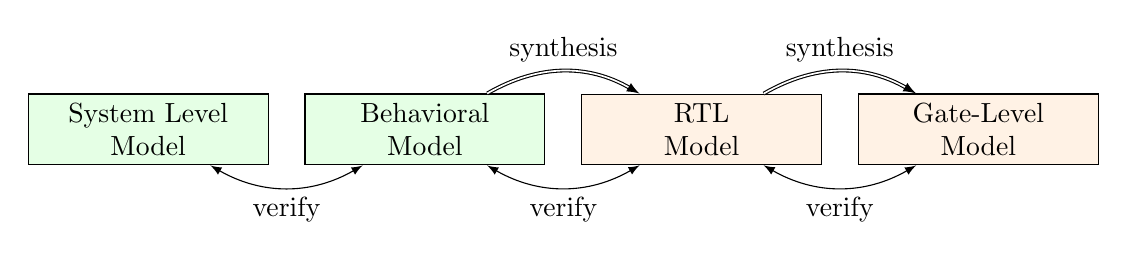
\begin{tikzpicture}
			\tikzstyle{manual} = [draw, fill=green!10, rectangle, minimum height=2em, minimum width=8em, node distance=10em]
			\tikzstyle{auto} = [draw, fill=orange!10, rectangle, minimum height=2em, minimum width=8em, node distance=10em]

			\node[manual] (sys) {\begin{minipage}{8em}
				\center
				System Level \\
				Model
			\end{minipage}};
			\node[manual] (beh) [right of=sys] {\begin{minipage}{8em}
				\center
				Behavioral \\
				Model
			\end{minipage}};
			\node[auto] (rtl) [right of=beh] {\begin{minipage}{8em}
				\center
				RTL \\
				Model
			\end{minipage}};
			\node[auto] (gates) [right of=rtl] {\begin{minipage}{8em}
				\center
				Gate-Level \\
				Model
			\end{minipage}};

			\draw[-latex] (beh) edge[double, bend left] node[above] {synthesis} (rtl);
			\draw[-latex] (rtl) edge[double, bend left] node[above] {synthesis} (gates);

			\draw[latex-latex] (sys) edge[bend right] node[below] {verify} (beh);
			\draw[latex-latex] (beh) edge[bend right] node[below] {verify} (rtl);
			\draw[latex-latex] (rtl) edge[bend right] node[below] {verify} (gates);
	\end{tikzpicture}
	\caption{Typical design flow. Green boxes represent manually created models. Orange boxes represent
	models generated by synthesis tools.}
	\label{fig:Basics_flow}
\end{figure}

In this example the System Level Model and the Behavioural Model are both
manually written design files. After the equivalence of system level model
and behavioural model has been verified, the lower level representations of the
design can be generated using synthesis tools. Finally the RTL Model and
the Gate-Level Model are verified and the design process is finished.

However, in any real-world design effort there will be multiple iterations for
this design process. The reason for this can be the late change of a design
requirement or the fact that the analysis of a low-abstraction model (e.g.~gate-level
timing analysis) revealed that a design change is required in order to meet
the design requirements (e.g.~maximum possible clock speed).

Whenever the behavioural model or the system level model is
changed their equivalence must be re-verified by re-running the simulations
and comparing the results. Whenever the behavioural model is changed the
synthesis must be re-run and the synthesis results must be re-verified.

In order to guarantee reproducibility it is important to be able to re-run all
automatic steps in a design project with a fixed set of settings easily.
Because of this, usually all programs used in a synthesis flow can be
controlled using scripts. This means that all functions are available via
text commands. When such a tool provides a gui, this is complementary to,
and not instead of, a command line interface.

Usually a synthesis flow in an UNIX/Linux environment would be controlled by a
shell script that calls all required tools (synthesis and simulation/verification
in this example) in the correct order. Each of these tools would be called with
a script file containing commands for the respective tool. All settings required
for the tool would be provided by these script files so that no manual interaction
would be necessary. These script files are considered design sources and should
be kept under version control just like the source code of the system level and the
behavioural model.

\section{Methods from Compiler Design}

Some parts of synthesis tools involve problem domains that are traditionally known from
compiler design. This section addresses some of these domains.

\subsection{Lexing and Parsing}

The best known concepts from compiler design are probably {\it lexing} and {\it parsing}.
These are two methods that together can be used to process complex computer languages
easily. \cite{Dragonbook}

A {\it lexer} consumes single characters from the input and generates a stream of {\it lexical
tokens} that consist of a {\it type} and a {\it value}. For example the Verilog input
``\lstinline[language=Verilog]{assign foo = bar + 42;}'' might be translated by the lexer
to the list of lexical tokens given in Tab.~\ref{tab:Basics_tokens}.

\begin{table}[t]
\hfil
\begin{tabular}{ll}
Token-Type & Token-Value \\
\hline
\tt TOK\_ASSIGN & - \\
\tt TOK\_IDENTIFIER & ``{\tt foo}'' \\
\tt TOK\_EQ & - \\
\tt TOK\_IDENTIFIER & ``{\tt bar}'' \\
\tt TOK\_PLUS & - \\
\tt TOK\_NUMBER & 42 \\
\tt TOK\_SEMICOLON & - \\
\end{tabular}
\caption{Exemplary token list for the statement ``\lstinline[language=Verilog]{assign foo = bar + 42;}''.}
\label{tab:Basics_tokens}
\end{table}

The lexer is usually generated by a lexer generator (e.g.~{\tt flex} \citeweblink{flex}) from a
description file that is using regular expressions to specify the text pattern that should match
the individual tokens.

The lexer is also responsible for skipping ignored characters (such as whitespace outside string
constants and comments in the case of Verilog) and converting the original text snippet to a token
value.

Note that individual keywords use different token types (instead of a keyword type with different
token values). This is because the parser usually can only use the Token-Type to make a decision on
the grammatical role of a token.

The parser then transforms the list of tokens into a parse tree that closely resembles the productions
from the computer languages grammar. As the lexer, the parser is also typically generated by a code
generator (e.g.~{\tt bison} \citeweblink{bison}) from a grammar description in Backus-Naur Form (BNF).

Let's consider the following BNF (in Bison syntax):

\begin{lstlisting}[numbers=left,frame=single]
assign_stmt: TOK_ASSIGN TOK_IDENTIFIER TOK_EQ expr TOK_SEMICOLON;
expr: TOK_IDENTIFIER | TOK_NUMBER | expr TOK_PLUS expr;
\end{lstlisting}

\begin{figure}[b!]
	\hfil
	\begin{tikzpicture}
			\tikzstyle{node} = [draw, fill=green!10, ellipse, minimum height=2em, minimum width=8em, node distance=10em]

			\draw (+0,+1) node[node] (n1) {\tt assign\_stmt};

			\draw (-6,-1) node[node] (n11) {\tt TOK\_ASSIGN};
			\draw (-3,-2) node[node] (n12) {\tt TOK\_IDENTIFIER};
			\draw (+0,-1) node[node] (n13) {\tt TOK\_EQ};
			\draw (+3,-2) node[node] (n14) {\tt expr};
			\draw (+6,-1) node[node] (n15) {\tt TOK\_SEMICOLON};

			\draw (-1,-4) node[node] (n141) {\tt expr};
			\draw (+3,-4) node[node] (n142) {\tt TOK\_PLUS};
			\draw (+7,-4) node[node] (n143) {\tt expr};

			\draw (-1,-5.5) node[node] (n1411) {\tt TOK\_IDENTIFIER};
			\draw (+7,-5.5) node[node] (n1431) {\tt TOK\_NUMBER};

			\draw[-latex] (n1) -- (n11);
			\draw[-latex] (n1) -- (n12);
			\draw[-latex] (n1) -- (n13);
			\draw[-latex] (n1) -- (n14);
			\draw[-latex] (n1) -- (n15);

			\draw[-latex] (n14) -- (n141);
			\draw[-latex] (n14) -- (n142);
			\draw[-latex] (n14) -- (n143);

			\draw[-latex] (n141) -- (n1411);
			\draw[-latex] (n143) -- (n1431);
	\end{tikzpicture}
	\caption{Example parse tree for the Verilog expression ``\lstinline[language=Verilog]{assign foo = bar + 42;}''.}
	\label{fig:Basics_parsetree}
\end{figure}

The parser converts the token list to the parse tree in Fig.~\ref{fig:Basics_parsetree}. Note that the parse
tree never actually exists as a whole as data structure in memory. Instead the parser calls user-specified
code snippets (so-called {\it reduce-functions}) for all inner nodes of the parse tree in depth-first order.

In some very simple applications (e.g.~code generation for stack machines) it is possible to perform the
task at hand directly in the reduce functions. But usually the reduce functions are only used to build an in-memory
data structure with the relevant information from the parse tree. This data structure is called an {\it abstract
syntax tree} (AST).

The exact format for the abstract syntax tree is application specific (while the format of the parse tree and token
list are mostly dictated by the grammar of the language at hand). Figure~\ref{fig:Basics_ast} illustrates what an
AST for the parse tree in Fig.~\ref{fig:Basics_parsetree} could look like.

Usually the AST is then converted into yet another representation that is more suitable for further processing.
In compilers this is often an assembler-like three-address-code intermediate representation. \cite{Dragonbook}

\begin{figure}[t]
	\hfil
	\begin{tikzpicture}
			\tikzstyle{node} = [draw, fill=green!10, ellipse, minimum height=2em, minimum width=8em, node distance=10em]

			\draw (+0,+0) node[node] (n1) {\tt ASSIGN};

			\draw (-2,-2) node[node] (n11) {\tt ID: foo};
			\draw (+2,-2) node[node] (n12) {\tt PLUS};

			\draw (+0,-4) node[node] (n121) {\tt ID: bar};
			\draw (+4,-4) node[node] (n122) {\tt CONST: 42};

			\draw[-latex] (n1) -- (n11);
			\draw[-latex] (n1) -- (n12);

			\draw[-latex] (n12) -- (n121);
			\draw[-latex] (n12) -- (n122);
	\end{tikzpicture}
	\caption{Example abstract syntax tree for the Verilog expression ``\lstinline[language=Verilog]{assign foo = bar + 42;}''.}
	\label{fig:Basics_ast}
\end{figure}

\subsection{Multi-Pass Compilation}

Complex problems are often best solved when split up into smaller problems. This is certainly true
for compilers as well as for synthesis tools. The components responsible for solving the smaller problems can
be connected in two different ways: through {\it Single-Pass Pipelining} and by using {\it Multiple Passes}.

Traditionally a parser and lexer are connected using the pipelined approach: The lexer provides a function that
is called by the parser. This function reads data from the input until a complete lexical token has been read. Then
this token is returned to the parser. So the lexer does not first generate a complete list of lexical tokens
and then pass it to the parser. Instead they run concurrently and the parser can consume tokens as
the lexer produces them.

The single-pass pipelining approach has the advantage of lower memory footprint (at no time must the complete design
be kept in memory) but has the disadvantage of tighter coupling between the interacting components.

Therefore single-pass pipelining should only be used when the lower memory footprint is required or the
components are also conceptually tightly coupled. The latter certainly is the case for a parser and its lexer.
But when data is passed between two conceptually loosely coupled components it is often
beneficial to use a multi-pass approach.

In the multi-pass approach the first component processes all the data and the result is stored in a in-memory
data structure. Then the second component is called with this data. This reduces complexity, as only one
component is running at a time. It also improves flexibility as components can be exchanged easier.

Most modern compilers are multi-pass compilers.

\iffalse
\subsection{Static Single Assignment Form}

In imperative programming (and behavioural HDL design) it is possible to assign the same variable multiple times.
This can either mean that the variable is independently used in two different contexts or that the final value
of the variable depends on a condition.

The following examples show C code in which one variable is used independently in two different contexts:

\begin{minipage}{7.7cm}
\begin{lstlisting}[numbers=left,frame=single,language=C++]
void demo1()
{
	int a = 1;
	printf("%d\n", a);

	a = 2;
	printf("%d\n", a);
}
\end{lstlisting}
\end{minipage}
\hfil
\begin{minipage}{7.7cm}
\begin{lstlisting}[frame=single,language=C++]
void demo1()
{
	int a = 1;
	printf("%d\n", a);

	int b = 2;
	printf("%d\n", b);
}
\end{lstlisting}
\end{minipage}

\begin{minipage}{7.7cm}
\begin{lstlisting}[numbers=left,frame=single,language=C++]
void demo2(bool foo)
{
	int a;
	if (foo) {
		a = 23;
		printf("%d\n", a);
	} else {
		a = 42;
		printf("%d\n", a);
	}
}
\end{lstlisting}
\end{minipage}
\hfil
\begin{minipage}{7.7cm}
\begin{lstlisting}[frame=single,language=C++]
void demo2(bool foo)
{
	int a, b;
	if (foo) {
		a = 23;
		printf("%d\n", a);
	} else {
		b = 42;
		printf("%d\n", b);
	}
}
\end{lstlisting}
\end{minipage}

In both examples the left version (only variable \lstinline[language=C++]{a}) and the right version (variables
\lstinline[language=Verilog]{a} and \lstinline[language=Verilog]{b}) are equivalent. Therefore it is
desired for further processing to bring the code in an equivalent form for both cases.

In the following example the variable is assigned twice but it cannot be easily replaced by two variables:

\begin{lstlisting}[frame=single,language=C++]
void demo3(bool foo)
{
	int a = 23
	if (foo)
		a = 42;
	printf("%d\n", a);
}
\end{lstlisting}

Static single assignment (SSA) form is a representation of imperative code that uses identical representations
for the left and right version of demos 1 and 2, but can still represent demo 3. In SSA form each assignment
assigns a new variable (usually written with an index). But it also introduces a special $\Phi$-function to
merge the different instances of a variable when needed. In C-pseudo-code the demo 3 would be written as follows
using SSA from:

\begin{lstlisting}[frame=single,language=C++]
void demo3(bool foo)
{
	int a_1, a_2, a_3;
	a_1 = 23
	if (foo)
		a_2 = 42;
	a_3 = phi(a_1, a_2);
	printf("%d\n", a_3);
}
\end{lstlisting}

The $\Phi$-function is usually interpreted as ``these variables must be stored
in the same memory location'' during code generation. Most modern compilers for imperative languages
such as C/C++ use SSA form for at least some of its passes as it is very easy to manipulate and analyse.
\fi

